\begin{frame}[t]{LoRa Frequency Plans and Regulation}

  \begin{itemize}
\item LoRa arbeitet im \alert{lizenzfreien ISM}-Band (Industrial/Scientific/Medical).
\item Aber dieses Frequenzband ist \alert{nicht unreguliert}! Man darf das Band \alert{nicht beliebig lange belegen}; die Airtime ist begrenzt.
\item \alert {Duty Cycle}: Maximal erlaubter Airtime-Anteil in Prozent (\%).
\item Regulierungen unterscheiden sich je nach Region der Welt.
  \end{itemize}
  \begin{center}
%    \only<1>{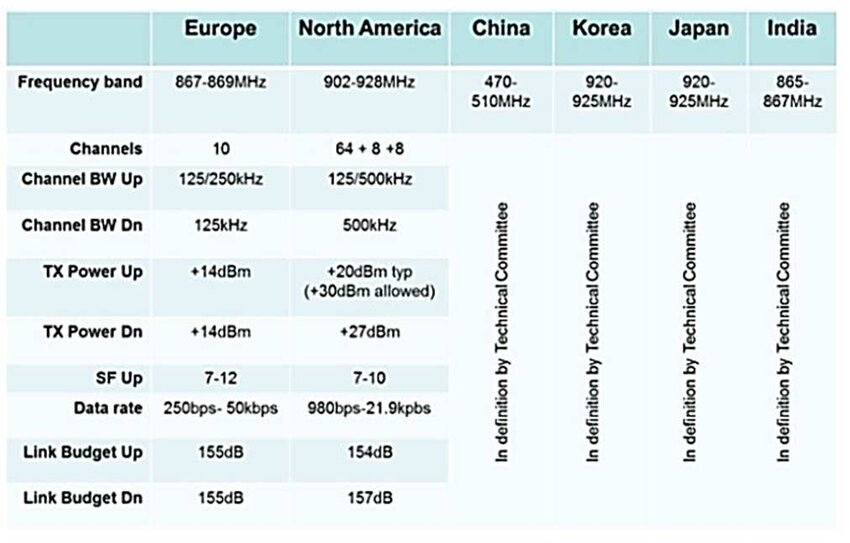
\includegraphics[width=0.6\textwidth]{material/LoRaWAN-Frequency-Allocation-14.png}}
    \only<1>{\begin{table}\begin{tabular}{r@{\ }c@{\ }l|r|r|r}
      \toprule
        \multicolumn{3}{r|}{Frequency}& Bandwidth & Duty Cycle & Power \\
        \multicolumn{3}{r|}{[$\SI{}{\mega\hertz}$]}&[$\SI{}{\kilo\hertz}$] & [\%] & [$\SI{}{\milli\watt}]$\\
      \midrule
        863 &--& 865 & 125, 250, 500 &$\num{0.1}$& $\num{25}$ \\
        865 &--& 868 & 125, 250, 500 &$\num{1.0}$& $\num{25}$\\
        868 &--& 868,6 & 125, 250, 500 &$\num{1.0}$& $\num{25}$\\
        868,7 &--& 869,2 & 125, 250, 500 &$\num{0.1}$& $\num{25}$\\
        869,4 &--& 869,65 & 125, 250, 500 &$\num{10.0}$& $\num{500}$\\
        869,7 &--& 870 & 125, 250, 500 &$\num{1.0}$& $\num{25}$
      \end{tabular}
      \caption{Regulierte Parameter in der EU (EU863–870)}\end{table}}
  \end{center}
\end{frame}
